\PassOptionsToPackage{dvipsnames,table}{xcolor}
\documentclass{article}

\usepackage{iclr2027_conference,times}
\input{math_commands.tex}

\usepackage{amsmath,bm}
\usepackage{booktabs,tabularx,longtable,multirow,array}
\usepackage{graphicx}
\usepackage[font=small,labelfont=bf]{caption}
\usepackage{subcaption}
\usepackage{xcolor}
\usepackage{enumitem}
\usepackage{hyperref}
\usepackage[nameinlink,noabbrev]{cleveref}
\usepackage{url}

\definecolor{PDEBlue}{HTML}{153B5B}
\definecolor{PDELight}{HTML}{E9EFF3}
\definecolor{PDEOrange}{HTML}{E07A3F}
\definecolor{PDERed}{HTML}{B84842}
\newcolumntype{Y}{>{\raggedright\arraybackslash}X}
\newcommand{\dataset}{\textsc{PDE-OBS}}
\providecommand{\R}{\mathbb{R}}
\newcommand{\norm}[1]{\left\lVert #1 \right\rVert}
\newcommand{\code}[1]{\texttt{#1}}
\newcommand{\obs}{\Omega_{\mathrm{obs}}}

\setlist[itemize]{leftmargin=1.5em,itemsep=2pt,topsep=3pt}
\setlist[enumerate]{leftmargin=1.7em,itemsep=2pt,topsep=3pt}
\captionsetup{belowskip=3pt}
\renewcommand{\arraystretch}{1.12}

\title{\dataset: A Benchmark Builder for Learning\\
PDE Dynamics from Partial Observations}

% Keep authors anonymous for the ICLR submission version.
\author{Anonymous Authors}

% \iclrfinalcopy
\begin{document}

\maketitle

\begin{abstract}
\end{abstract}

% The main paper body is intentionally left empty at this stage.

\clearpage
\bibliographystyle{iclr2027_conference}
\bibliography{references}

\clearpage
\appendix
\def\PDEOBSAPPENDIXINPUT{1}
\ifdefined\PDEOBSAPPENDIXINPUT
\else
\documentclass[10pt]{article}

\usepackage[letterpaper,margin=0.82in]{geometry}
\usepackage[T1]{fontenc}
\usepackage{newtxtext,newtxmath}
\usepackage{microtype}
\usepackage{amsmath,bm}
\usepackage{booktabs,tabularx,longtable,multirow,array}
\usepackage{graphicx}
\usepackage[font=small,labelfont=bf]{caption}
\usepackage{subcaption}
\usepackage[dvipsnames,table]{xcolor}
\usepackage{enumitem}
\usepackage{natbib}
\usepackage[colorlinks=true,allcolors=NavyBlue]{hyperref}
\usepackage[nameinlink,noabbrev]{cleveref}

\definecolor{PDEBlue}{HTML}{153B5B}
\definecolor{PDELight}{HTML}{E9EFF3}
\definecolor{PDEOrange}{HTML}{E07A3F}
\definecolor{PDERed}{HTML}{B84842}
\newcolumntype{Y}{>{\raggedright\arraybackslash}X}
\newcommand{\dataset}{\textsc{PDE-OBS}}
\newcommand{\R}{\mathbb{R}}
\newcommand{\norm}[1]{\left\lVert #1 \right\rVert}
\newcommand{\code}[1]{\texttt{#1}}
\newcommand{\obs}{\Omega_{\mathrm{obs}}}

\setlist[itemize]{leftmargin=1.5em,itemsep=2pt,topsep=3pt}
\setlist[enumerate]{leftmargin=1.7em,itemsep=2pt,topsep=3pt}
\captionsetup{belowskip=3pt}
\renewcommand{\arraystretch}{1.12}

\title{\vspace{-1.0cm}\textbf{\dataset: A Benchmark Builder for Learning PDE Dynamics from Partial Observations}\\[2mm]
\large Supplementary Material --- Appendix A--D}
\author{PDE-OBS Contributors}
\date{}

\begin{document}
\maketitle
\vspace{-1.2em}

\begin{abstract}
This supplement specifies the scope, metrics, experimental contract, governing
equations, and numerical routes of \dataset.  Its organization follows the
role of Appendices A--D in the PDEBench supplement \citep{takamoto2022pdebench},
while the benchmark design and all descriptions here are specific to partial
observation.  The central artifact is a benchmark builder that factorizes
physical systems, boundary conditions, data-generating settings, difficulty
regimes, and sensing operators.  Ground truth is always generated before an
observation mask is applied.  This ordering makes it possible to separate
solver validity from reconstruction quality and to compare matched-mask and
mask-transfer performance without changing the underlying dynamics.
\end{abstract}

\noindent\colorbox{PDELight}{\parbox{0.965\linewidth}{\textbf{Status of the evidence.}
The numerical values reported in this appendix are from the checked-in
20-sample-per-factor solver preflight (5,600 samples).  They validate the
implemented discrete routes against their operator-matched residuals.  They
are neither learned-model results nor an independent grid-convergence study.
The full T15 dataset campaign stores 15 temporal frames and is evaluated by a
separate strict aggregate quality check.}}

\appendix
\fi

\section{Benchmark context and continuation of related work}
\label{sec:context}

\subsection{From full-field simulation benchmarks to partial observation}

Scientific machine learning benchmarks commonly assume that the state is
available on the complete computational grid.  PDEBench established a broad
multi-equation benchmark for forward simulation, inverse problems, and
standardized errors \citep{takamoto2022pdebench}.  Operator-learning methods
such as DeepONet \citep{lu2021deeponet}, the Fourier Neural Operator (FNO)
\citep{li2021fno}, the Convolutional Neural Operator (CNO)
\citep{kovachki2023cno}, and physics-informed neural operators
\citep{li2021pino} provide strong function-to-function modeling primitives.
Physics-informed neural networks instead optimize a coordinate-based solution
under data and residual constraints \citep{raissi2019pinns}.  These lines of
work motivate the model families represented in the \dataset method catalog,
but do not by themselves define a controlled sensing benchmark.

Partial observation adds a distinct statistical axis.  A model may see random
point sensors, installed grids, lines, boundaries, clustered instruments, or a
field with a missing region.  Generative methods such as DiffusionPDE
\citep{tang2024diffusionpde} and functional posterior-sampling approaches such
as FunDPS \citep{chung2025fundps} directly target conditional field recovery.
However, comparing such approaches requires more than collecting several
sparse-input experiments: the physical sample, the sensing process, the data
split, and the evaluation mask must be held under an explicit contract.

\subsection{The \dataset contribution}

The primary contribution is the \emph{benchmark builder and protocol}, not a
new neural architecture.  A benchmark instance is represented as
\begin{equation}
  \mathcal{B} = \mathcal{P}\times\mathcal{B}_{\partial}
  \times\mathcal{S}\times\mathcal{R}\times\mathcal{M},
  \label{eq:factorization}
\end{equation}
where $\mathcal{P}$ is the PDE family, $\mathcal{B}_{\partial}$ the boundary
protocol, $\mathcal{S}$ the field-generating setting, $\mathcal{R}$ the
physical regime, and $\mathcal{M}$ the observation protocol.  The released
core contains seven PDEs, four boundary protocols, ten settings, three
regimes, and nine masks.  The physical Cartesian product contains
$7\times4\times10=280$ macro cases and 840 regime nodes.  Observation masks
are sampled downstream and therefore do not multiply the stored ground-truth
simulation pool.

This design supports four questions that are otherwise easily conflated:
\begin{enumerate}
  \item \textbf{Physical generalization:} does performance transfer across
  PDEs, parameters, or boundaries?
  \item \textbf{Observation generalization:} does a model trained on one
  sensor geometry transfer to another?
  \item \textbf{Resolution and horizon behavior:} does error remain controlled
  across spatial frequencies and rollout time?
  \item \textbf{Numerical validity:} was the target field accepted before any
  learned method saw it?
\end{enumerate}

The benchmark records method capabilities separately from method availability.
The compact RBF, U-Net, FNO, and CNO adapters are executable in the current
codebase; other catalog entries may be planning-only.  A planning entry is not
silently treated as a runnable baseline.  Likewise, the current full-campaign
phase is dataset generation and quality control only; training results are not
claimed in this supplement.

\subsection{Design principles}

\paragraph{Ground truth precedes sensing.}
For a seed $s$, the generator first produces the complete field or trajectory
$u_s$.  Only then is a mask $m$ drawn and applied:
\begin{equation}
  y_s = m\odot u_s + \eta,
  \qquad m\in\{0,1\}^{H\times W}.
\end{equation}
Consequently, changing a mask never changes the PDE solver, coefficients,
initial condition, or target trajectory.  The present deterministic benchmark
uses $\eta=0$ by default; controlled noise can be added as an evaluation
extension without regenerating $u_s$.

\paragraph{Matched-mask and transfer results are separate.}
The primary comparison trains and tests a method under the same named mask.
The secondary mask-transfer experiment trains on the canonical random-3\%
protocol and evaluates all other masks.  Pooling both settings into one table
would hide whether a gain comes from better reconstruction or familiarity with
the sensor layout.

\paragraph{Every result is tied to provenance.}
Configurations resolve into immutable generation plans containing seeds,
factor labels, solver options, expected shapes, and output paths.  Completed
shards carry metadata, quality records, and SHA-256 checksums.  Git commit,
environment specification, plan row, and data checksum together define the
reproduction unit.

\section{Detailed metrics and observation protocol}
\label{sec:metrics}

\subsection{Notation and evaluation domain}

Let $u\in\R^{T\times H\times W\times V}$ be the accepted target and
$\widehat{u}$ a prediction.  Static equations use $T=1$.  The binary sensor
mask $m\in\{0,1\}^{H\times W}$ is broadcast over time and channels.  We report
metrics on the full target domain unless the metric name explicitly carries
the suffix ``observed'' or ``unobserved.''  For any subset $A$, let
$|A|$ denote the number of scalar entries after time/channel broadcasting.

\subsection{Pointwise and normalized field errors}

The mean-squared and mean-absolute errors are
\begin{align}
  \mathrm{MSE}(\widehat{u},u)
    &= \frac{1}{N}\sum_{i=1}^{N}(\widehat{u}_i-u_i)^2,\\
  \mathrm{MAE}(\widehat{u},u)
    &= \frac{1}{N}\sum_{i=1}^{N}|\widehat{u}_i-u_i|.
\end{align}
The per-sample relative $L_2$ error is
\begin{equation}
  E_{L_2}^{(n)} =
  \frac{\norm{\widehat{u}^{(n)}-u^{(n)}}_2}
       {\norm{u^{(n)}}_2+\varepsilon},
  \label{eq:rel-l2}
\end{equation}
and is aggregated across samples rather than after concatenating the batch.
This prevents high-amplitude regimes from dominating every comparison.
Subset metrics use the same formulas with indices restricted to
$A=\obs$ or $A=\Omega\setminus\obs$.

\subsection{Spectral, temporal, and physical diagnostics}

Spatial averages alone can hide the loss of small scales.  For each field, the
implementation computes a two-dimensional discrete Fourier transform over the
spatial axes and partitions normalized radial frequency into low, middle, and
high bands.  With radial Nyquist $r_{\max}=\sqrt{1/2}$, the default intervals
are $[0,r_{\max}/3)$, $[r_{\max}/3,2r_{\max}/3)$, and
$[2r_{\max}/3,r_{\max}]$.  The band-relative error is
\begin{equation}
  E_b = \frac{\norm{\mathbf{1}_b(\widehat{U}-U)}_2}
  {\norm{\mathbf{1}_b U}_2+\varepsilon},
  \label{eq:spectral-band}
\end{equation}
where $U=\mathcal{F}_{xy}(u)$ and $\mathbf{1}_b$ selects band $b$.  Spectral
centroid and high-frequency energy are additionally recorded to diagnose
over-smoothing.

For dynamic systems, errors are evaluated by stored frame and summarized at
rollout horizons $1$, $2$, $4$, and $8$ when those horizons exist.  Kinetic
energy, vorticity, and enstrophy diagnostics are reported for compatible flow
states.  Stability reporting counts non-finite values and trajectories that
leave documented physical ranges; it is not replaced by a visually plausible
final frame.

\begin{table}[t]
\centering
\caption{Metric groups and their role in a partial-observation benchmark.}
\label{tab:metrics}
\small
\begin{tabularx}{\linewidth}{@{}p{0.18\linewidth}p{0.28\linewidth}Y@{}}
\toprule
Group & Representative outputs & Interpretation \\
\midrule
Field error & MSE, MAE, relative $L_2$ & Overall reconstruction fidelity on full, observed, or unobserved domains. \\
Spectral error & Low/mid/high $E_b$, centroid, high-frequency energy & Whether fine structures are recovered rather than smoothed away. \\
Rollout & Per-frame error; horizons 1, 2, 4, 8 & Accumulation of temporal error and long-horizon stability. \\
Physics & Energy, vorticity, enstrophy, residual diagnostics & Preservation of known invariants or PDE-compatible structure. \\
Robustness & OOD degradation; mask-transfer gap & Sensitivity to regimes and sensing layouts not used for fitting. \\
Data quality & Normalized discrete PDE loss & Acceptance of generated ground truth; never a model-score substitute. \\
\bottomrule
\end{tabularx}
\end{table}

\subsection{Nine observation protocols}

At $128\times128$, \dataset uses the deterministic realized counts in
\cref{tab:masks}.  Random masks select distinct pixels without replacement.
The regular grid uses fixed spacing, the line mask uses horizontal and
vertical transects, boundary sensors lie on the exterior grid, and clustered
sensors sample from a mixture of localized kernels.  The missing-block
protocol is intentionally dense outside its hidden square: its difficulty is
structured extrapolation rather than extreme sparsity.

\begin{table}[t]
\centering
\caption{Official observation masks at $128\times128$; ``observed'' means
available to the reconstruction method.}
\label{tab:masks}
\small
\begin{tabular}{@{}lrrl@{}}
\toprule
Protocol & Observed pixels & Observed fraction & Structural feature \\
\midrule
Random 1\% & 164 & 1.00\% & Uniform distinct point sensors \\
Random 3\% & 500 & 3.05\% & Canonical training/transfer mask \\
Random 5\% & 819 & 5.00\% & Uniform distinct point sensors \\
Random 10\% & 1,638 & 10.00\% & Uniform distinct point sensors \\
Regular grid & 441 & 2.69\% & Installed lattice \\
Missing block & 12,288 & 75.00\% & One contiguous hidden quarter \\
Line sensors & 508 & 3.10\% & Two horizontal and two vertical lines \\
Boundary sensors & 508 & 3.10\% & Exterior-grid perimeter \\
Clustered sensors & 492 & 3.00\% & Four localized sensor groups \\
\bottomrule
\end{tabular}
\end{table}

\begin{figure}[p]
  \centering
  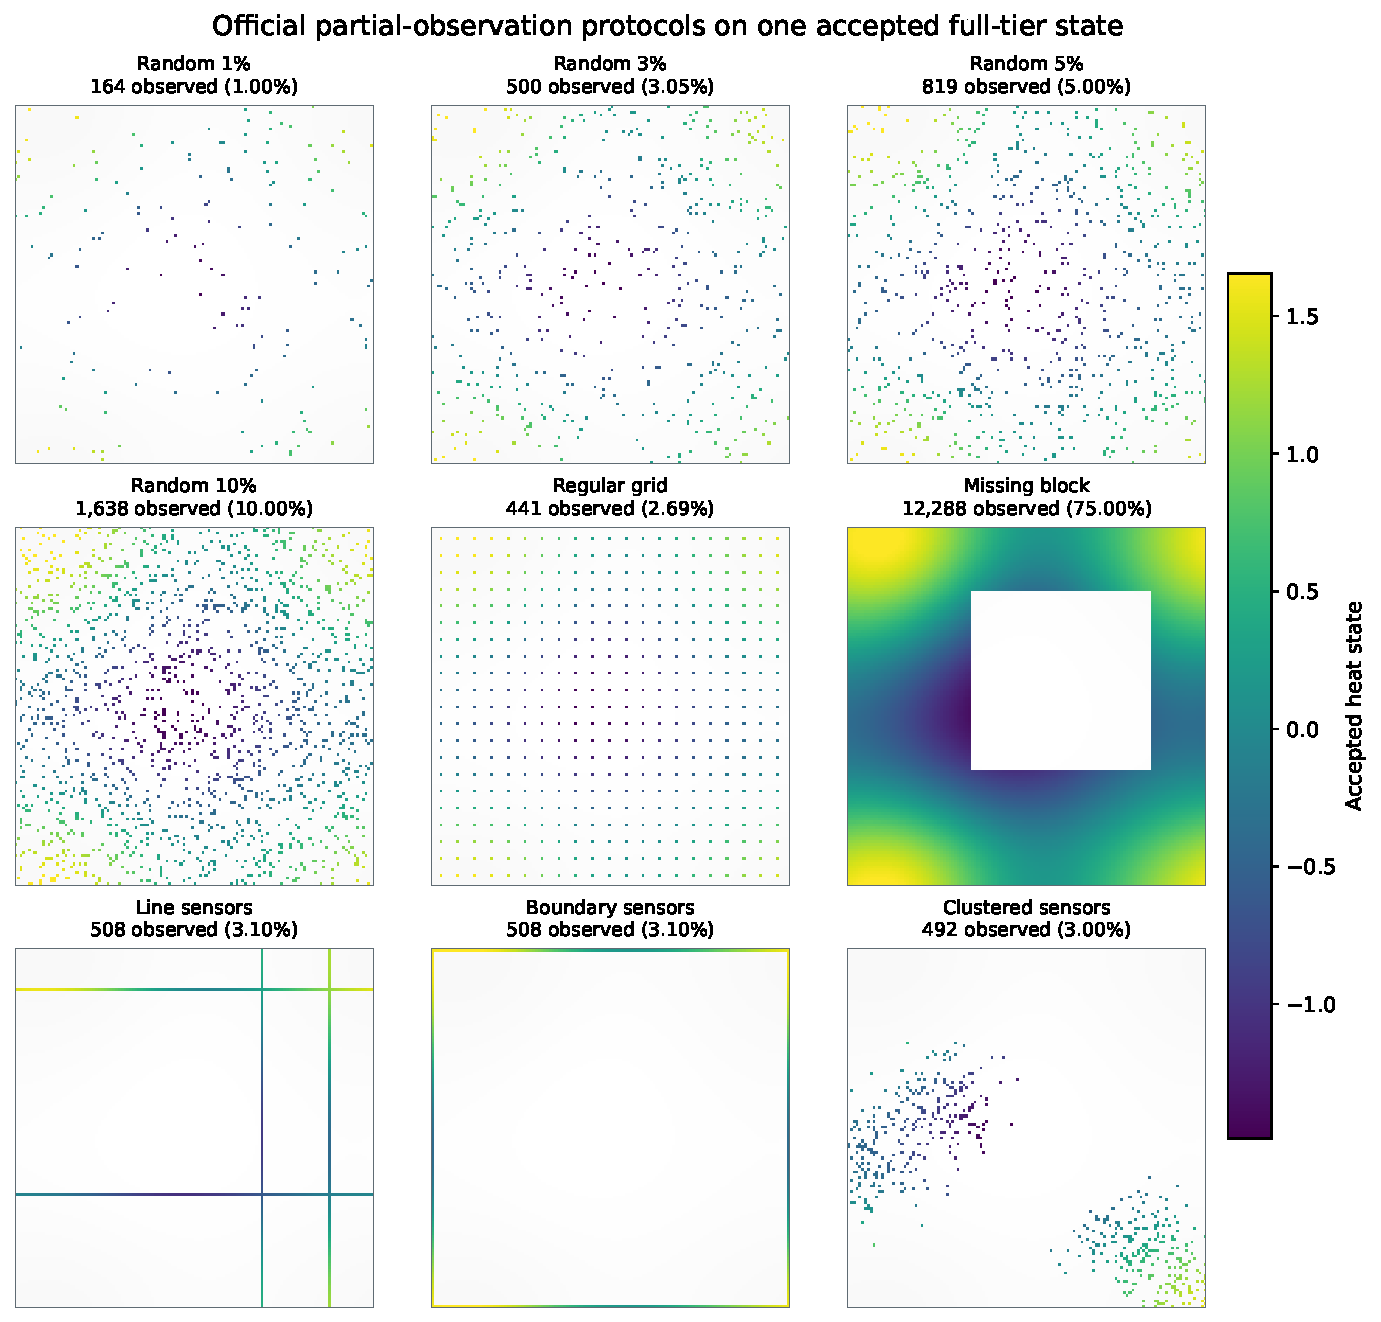
\includegraphics[width=0.92\linewidth]{figures/fig_observation_protocols.pdf}
  \caption{The nine official sensing protocols applied to the \emph{same}
  accepted full-tier heat-equation state stored on SeaWulf.  The faint field
  shows unobserved context for explanation only; a benchmark method receives
  values at the colored observed locations.  Counts are generated from the
  public mask implementations with fixed seeds.}
  \label{fig:masks}
\end{figure}

\subsection{Solver quality loss versus prediction loss}

Dataset acceptance and learned-model evaluation are deliberately separate.
For a generated field $u_h$, the quality module applies the discrete operator
$\mathcal{L}_h$ matched to the recorded solver route and constructs a
normalized residual
\begin{equation}
  \mathcal{Q}_{\mathrm{PDE}}
  = \frac{\norm{\mathcal{L}_h(u_h)-f_h}_2}
  {\norm{f_h}_2+\norm{\mathcal{L}_h(u_h)}_2+\varepsilon}.
  \label{eq:pde-loss}
\end{equation}
Temporal equations use the corresponding time-discrete replay or semigroup
contract and exclude the initial frame from one-step residual summaries.  A
shard is accepted only if every required record is finite and the configured
maximum is no greater than $0.05$.  By contrast, MSE and
\cref{eq:rel-l2,eq:spectral-band} compare a model prediction with an already
accepted target.  A low $\mathcal{Q}_{\mathrm{PDE}}$ therefore cannot be cited
as evidence of accurate reconstruction.

\section{Benchmark protocol, hyperparameters, and tools}
\label{sec:protocol}

\subsection{Dataset factorization and sample allocation}

\begin{table}[t]
\centering
\caption{Released benchmark axes.  Boundary and setting labels are semantic
contracts; each resolved plan records their exact normalized identifiers.}
\label{tab:factors}
\small
\begin{tabularx}{\linewidth}{@{}p{0.16\linewidth}p{0.08\linewidth}Y@{}}
\toprule
Axis & Count & Members \\
\midrule
PDE family & 7 & Darcy, Poisson, Helmholtz, heat, reaction--diffusion, Burgers, Navier--Stokes \\
Boundary & 4 & Dirichlet/no-slip; Neumann/free-slip; periodic; Robin/mixed obstacle \\
Setting & 10 & Smooth, medium, rough GRF; low- and multi-frequency Fourier; Gaussian blobs; piecewise blocks; threshold level set; dipole/vortex pair; front/ring/shock \\
Regime & 3 & Low, medium, high physical difficulty \\
Observation & 9 & Four random densities; grid; missing block; lines; boundary; clusters \\
\bottomrule
\end{tabularx}
\end{table}

The full tier allocates 2,000 samples to each of the 280 PDE--boundary--setting
macro cases, or 560,000 samples total.  Counts are split as evenly as possible
over low, medium, and high regimes while preserving deterministic seed ranges.
The current T15 campaign uses shards of at most 200 samples, producing 3,360
planned HDF5 shards.  Static equations store one state.  Dynamic equations
generate a denser in-memory trajectory for solver-quality checks and retain
exactly 15 uniformly spaced solver frames over the physical horizon.

\subsection{Canonical arrays and split contract}

Every unbatched record uses channels-last arrays:
\begin{align}
  \texttt{condition}&\in\R^{H\times W\times V_{\mathrm{cond}}},\\
  \texttt{trajectory}&\in\R^{T\times H\times W\times V_{\mathrm{state}}},\\
  \texttt{geometry}&\in\R^{H\times W\times 1}.
\end{align}
The first array contains a coefficient, source, or initial state according to
the PDE.  The trajectory is the target.  Geometry records domain support and
obstacles independently of sensor visibility.  Batched HDF5 arrays prepend the
sample dimension $N$.

Samples are assigned to deterministic IID train/validation/test splits in the
ratio 70/15/15 without reusing a seed across splits.  Published OOD studies
must additionally identify which factor is held out.  A method may fit only on
the training pool; validation controls selection, and the test pool is read
only for final evaluation.  The main sparse-recovery table uses matched masks.
The separate transfer table fits with random 3\% observations and evaluates all
nine protocols.

\subsection{Method-facing protocol}

For each accepted target, the data layer constructs
\begin{equation}
  x = \bigl(m\odot c,\ m,\ g,\ \theta\bigr),
  \qquad \widehat{u}=F_{\phi}(x),
\end{equation}
where $c$ is the observable condition/state, $g$ is geometry, and $\theta$
contains declared physical parameters.  The mask is supplied explicitly so
that a zero-valued measurement is not confused with an unobserved pixel.
Methods must declare whether they use coordinates, physics residuals, test-time
optimization, or posterior samples.  Stochastic methods report the number of
samples and the aggregation rule.  Test-time fitting cost is reported
separately from amortized inference.

\begin{table}[t]
\centering
\caption{Reproducibility controls enforced by the builder.}
\label{tab:repro-controls}
\small
\begin{tabularx}{\linewidth}{@{}p{0.23\linewidth}Y@{}}
\toprule
Control & Recorded information \\
\midrule
Resolved plan & Factor labels, sample counts, seeds, shapes, solver route, time grid, output path \\
Data shard & HDF5 arrays, schema version, per-sample metadata, atomic completion marker \\
Quality & Per-sample diagnostics, failure JSONL, strict aggregate CSV/JSON, threshold policy \\
Integrity & SHA-256 digest and manifest for each completed shard \\
Software & Git commit, Python environment, package constraints, command line, Slurm job identity \\
Method run & Method configuration, fit scope, mask protocol, checkpoint and evaluation outputs \\
\bottomrule
\end{tabularx}
\end{table}

\subsection{Numerical and workflow toolchain}

Generation is implemented in Python 3.11 with NumPy for array and Fourier
operations, SciPy for sparse linear algebra and sine transforms, h5py for HDF5
storage, and PyYAML for resolved configuration.  The generation-only
environment pins minimum versions NumPy 1.24, SciPy 1.10, h5py 3.8, and PyYAML
6.0.  Matplotlib is used only for analysis figures.  PyTorch is an optional
training dependency and is not required for dataset generation.

SeaWulf campaigns use Slurm arrays.  One plan row is serial within the current
generator, so a shard requests one CPU and approximately 4~GiB unless measured
evidence justifies more.  Parallelism comes from mutually exclusive array
elements rather than assigning an unused whole node to one shard.  Each writer
owns a distinct output path; atomic temporary files are promoted only after
quality and checksum completion.  Data, environments, caches, runs, and logs
are placed under the user's scratch allocation.  Accepted artifacts must be
copied to independent archival storage because scratch is not a backup.

\subsection{Numerical preflight}

Before the full tier, the validation20 campaign evaluated all
$7\times4\times10$ macro cases with 20 samples each: 840 shards and 5,600
samples.  All required records completed and all seven PDE maxima were below
the strict 0.05 gate.  The campaign occupied 27~GiB.  These results support
implementation readiness of the recorded routes, subject to the interpretation
boundary following \cref{eq:pde-loss}.  The release record marks independent
publication validation as incomplete.  Separately, \cref{fig:full-quality}
summarizes the accepted full-T15 shards available at the recorded SeaWulf
snapshot; it is not a substitute for the final frozen-plan aggregate.

\begin{figure}[t]
  \centering
  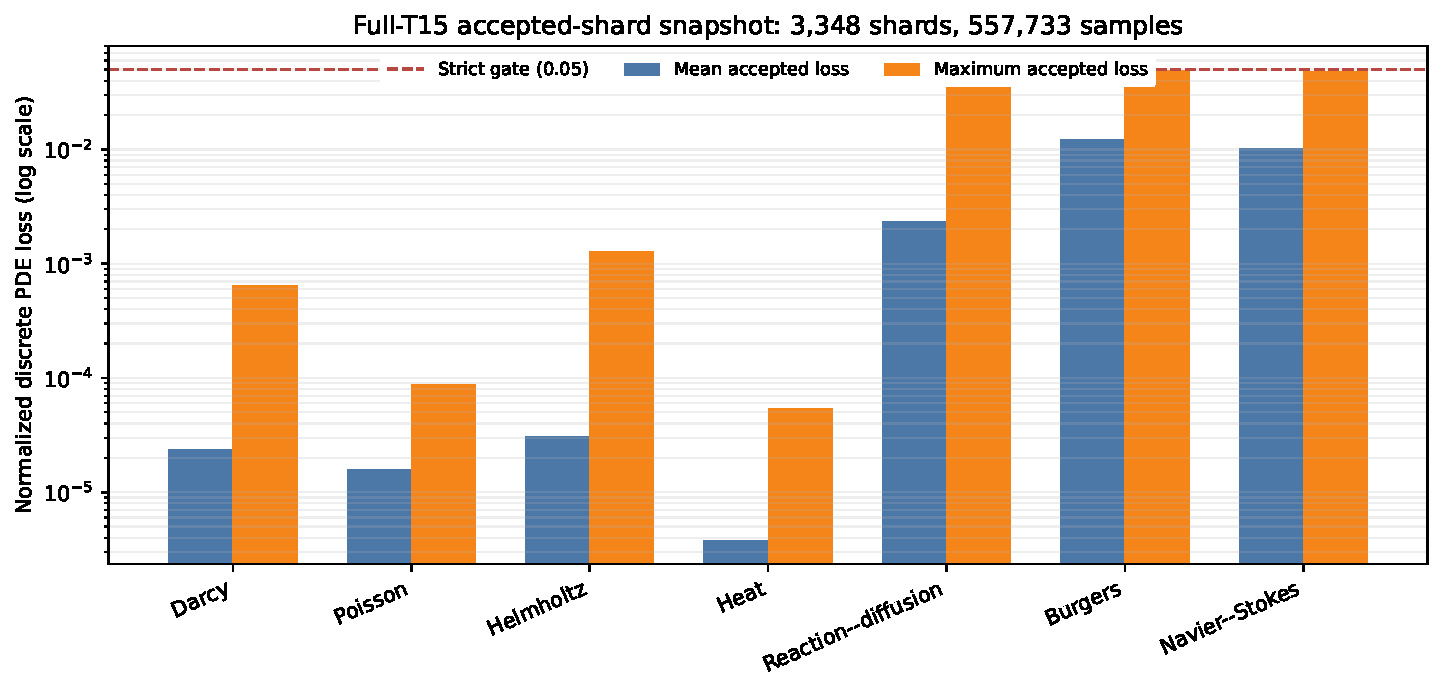
\includegraphics[width=0.92\linewidth]{figures/fig_full_quality_snapshot.pdf}
  \caption{Mean and maximum normalized discrete PDE loss over completed,
  accepted full-T15 shards at the SeaWulf rendering snapshot.  The dashed line
  is the strict 0.05 gate.  Rejected or absent shards are excluded by
  construction, so this descriptive snapshot is neither the final strict
  aggregate nor a learned-model result.}
  \label{fig:full-quality}
\end{figure}

\section{Detailed PDE and numerical-solver descriptions}
\label{sec:pdes}

\subsection{Common domain, boundaries, and regime semantics}

Unless otherwise stated, equations are posed on the unit square
$\Omega=[0,1]^2$ and discretized on a uniform $128\times128$ grid for released
data.  Four boundary labels provide a common experimental axis:
\begin{itemize}
  \item \textbf{Dirichlet/no-slip:} scalar values are fixed at the boundary;
  the flow route imposes no-slip walls through streamfunction and wall
  vorticity conditions.
  \item \textbf{Neumann/free-slip:} scalar normal derivatives vanish; the flow
  route uses a free-slip rectangular-wall formulation.
  \item \textbf{Periodic:} opposite edges are identified and derivatives are
  represented spectrally when the PDE route permits.
  \item \textbf{Robin/mixed obstacle:} scalar operators use the registered
  mixed boundary discretization; flow uses a true fluid mask, an internal
  obstacle, and wall-vorticity closure.
\end{itemize}
The low/medium/high regimes change a physically meaningful coefficient, not a
generic post-hoc noise level.  Parameter values are summarized in
\cref{tab:pde-parameters}.  The ten setting generators change spatial
regularity and topology of coefficients, sources, or initial states while
seeds remain local and deterministic.

\begin{table}[t]
\centering
\caption{Physical regime parameters and horizons.  ``Static'' equations store
one solution.}
\label{tab:pde-parameters}
\small
\begin{tabularx}{\linewidth}{@{}p{0.20\linewidth}p{0.30\linewidth}p{0.20\linewidth}Y@{}}
\toprule
PDE & Low / medium / high & Horizon & Stored state \\
\midrule
Darcy & coefficient contrast $2/8/32$ & static & pressure/head $u$ \\
Poisson & source amplitude $0.5/1/2$ & static & potential $u$ \\
Helmholtz & wavenumber $0.5/1/2$ & static & real field $u$ \\
Heat & diffusivity $0.005/0.02/0.08$ & $t_f=0.25$ & scalar $u$ \\
Reaction--diffusion & reaction rate $0.5/1.5/4$; $D=0.008$ & $t_f=0.8$ & scalar $u$ \\
Burgers & viscosity $0.04/0.015/0.004$ & $t_f=0.35$ & scalar $u$ \\
Navier--Stokes & viscosity $0.02/0.008/0.0025$; vorticity scale $2/3/4$ & $t_f=0.4$ & vorticity $\omega$ \\
\bottomrule
\end{tabularx}
\end{table}

\subsection{Darcy flow}

The heterogeneous Darcy problem is
\begin{equation}
  -\nabla\cdot\bigl(a(\bm{x})\nabla u(\bm{x})\bigr)=f(\bm{x}),
  \qquad \bm{x}\in\Omega.
  \label{eq:darcy}
\end{equation}
The setting generator produces a latent field that is range-normalized before
exponentiation, so the realized coefficient contrast equals the requested
regime rather than depending on the latent marginal distribution.  The source
is a fixed compatible zero-mean mixture of sine modes.  A face-flux
finite-volume operator preserves coefficient jumps, and the sparse system is
solved by a Krylov method with relative tolerance $10^{-9}$.  Periodic and
Neumann systems apply the appropriate compatibility and gauge treatment.  The
condition channel stores $a$; the target stores $u$.

\subsection{Poisson equation}

The Poisson family solves
\begin{equation}
  -\Delta u(\bm{x})=f(\bm{x}).
  \label{eq:poisson}
\end{equation}
The selected setting defines $f$, scaled by the regime amplitude.  The solver
uses a second-order flux-form finite-difference operator and a sparse Krylov
solve with relative tolerance $10^{-9}$.  Periodic sources are made zero mean;
Neumann sources are adjusted on the interior degrees of freedom to satisfy the
discrete compatibility condition.  The source is preserved in the condition
channel so an independent evaluator can reconstruct the stated right-hand
side.

\subsection{Helmholtz equation}

The real, undamped boundary-value problem is
\begin{equation}
  \left(-\Delta-k^2\right)u(\bm{x})=f(\bm{x}),
  \label{eq:helmholtz}
\end{equation}
with $k\in\{0.5,1,2\}$.  It is discretized with the same boundary-aware
second-order operator and solved as a real sparse system to relative tolerance
$10^{-9}$.  In particular, the periodic route does not take the real part of
a damped complex transfer function: that would solve a different equation.
The condition stores $f$, and the target stores $u$.

\subsection{Heat equation}

The heat equation is
\begin{equation}
  \partial_t u = D\Delta u, \qquad u(\bm{x},0)=u_0(\bm{x}).
  \label{eq:heat}
\end{equation}
For periodic boundaries, every Fourier mode is advanced by the exact diffusion
semigroup over the requested interval.  Bounded domains use a second-order
finite-difference Laplacian and Crank--Nicolson time integration with the
registered boundary equations included in the implicit solve.  Thus the wall
values are not overwritten after a periodic update.  The condition and first
trajectory frame both encode $u_0$; full T15 records contain 15 ordered frames.

\subsection{Reaction--diffusion equation}

The scalar Allen--Cahn-type system is
\begin{equation}
  \partial_t u = D\Delta u+r(u-u^3),
  \qquad D=0.008.
  \label{eq:reaction}
\end{equation}
The route uses Strang splitting.  The nonlinear reaction subproblem is advanced
with its exact pointwise flow for a half step, diffusion advances a full step,
and the exact reaction flow completes the interval.  Diffusion uses a Fourier
semigroup for periodic domains and a boundary-aware Crank--Nicolson solve for
bounded domains.  Adaptive internal substeps control the reaction update while
the stored frames remain uniformly spaced over $t\in[0,0.8]$.

\subsection{Two-dimensional scalar Burgers equation}

The benchmark uses the scalar two-dimensional conservation law
\begin{equation}
  \partial_t u + u(\partial_x u+\partial_y u)=\nu\Delta u.
  \label{eq:burgers}
\end{equation}
For smooth periodic settings, advection is computed pseudospectrally with the
$2/3$ de-aliasing rule.  Discontinuous settings and bounded domains use a
conservative local Lax--Friedrichs/Rusanov flux with SSP-RK2.  Both routes
choose internal steps from a two-dimensional CFL bound; diffusion is advanced
implicitly by the Fourier or boundary finite-difference route.  This
case-dependent selection prevents Gibbs-dominated spectral evolution of the
piecewise, threshold, and front/ring/shock settings.

\subsection{Incompressible Navier--Stokes equation}

The stored state is scalar vorticity $\omega$ for the two-dimensional
incompressible system
\begin{align}
  \partial_t\omega + \bm{v}\cdot\nabla\omega
    &= \nu\Delta\omega + f, \\
  -\Delta\psi &= \omega, \\
  \bm{v} &= (\partial_y\psi,-\partial_x\psi).
  \label{eq:navier-stokes}
\end{align}
The forcing is a fixed sine--cosine pattern and the initial vorticity is
setting-conditioned.  Boundary topology determines the complete solver:
\begin{itemize}
  \item \textbf{Periodic:} an FNO-style vorticity--streamfunction
  pseudospectral method with $2/3$ de-aliasing, Crank--Nicolson viscosity, and
  internal step $10^{-4}$.
  \item \textbf{No-slip and free-slip rectangles:} a discrete-sine-transform
  diagonalization for the bounded streamfunction, wall-vorticity update, and
  SSP-RK2 transport.
  \item \textbf{Obstacle domain:} a sparse Poisson solve on the true fluid
  mask, Thom-type wall/obstacle vorticity, and SSP-RK2 transport.
\end{itemize}
No bounded route performs a periodic evolution followed by boundary
overwriting.  This is essential because such overwriting can make images look
bounded while leaving the interior dynamics inconsistent with the stated
boundary-value problem.

\begin{table}[p]
\centering
\caption{Boundary-aware numerical route map.  ``FD2'' denotes a second-order
finite-difference/flux discretization; ``CN'' denotes Crank--Nicolson.}
\label{tab:solver-map}
\small
\begin{tabularx}{\linewidth}{@{}p{0.16\linewidth}p{0.18\linewidth}Y@{}}
\toprule
PDE & Boundary class & Numerical route \\
\midrule
Darcy & all four & Variable-coefficient face-flux finite volume; sparse Krylov BVP solve \\
Poisson & all four & Boundary-aware FD2 flux operator; compatibility/gauge handling; sparse Krylov solve \\
Helmholtz & all four & Real undamped FD2 Helmholtz operator; sparse Krylov solve \\
Heat & periodic & Exact Fourier diffusion semigroup \\
Heat & bounded/mixed & FD2 boundary operator with CN \\
Reaction--diffusion & periodic & Exact reaction--Fourier diffusion Strang splitting \\
Reaction--diffusion & bounded/mixed & Exact reaction--FD2/CN Strang splitting \\
Burgers & smooth periodic & $2/3$-dealiased pseudospectral advection with implicit diffusion \\
Burgers & discontinuous/\newline bounded & Rusanov flux, SSP-RK2, adaptive CFL, implicit diffusion \\
Navier--Stokes & periodic & Dealiased spectral vorticity--streamfunction; CN viscosity \\
Navier--Stokes & no-slip/free-slip & DST streamfunction, wall vorticity, SSP-RK2 \\
Navier--Stokes & obstacle & Masked sparse streamfunction, Thom wall vorticity, SSP-RK2 \\
\bottomrule
\end{tabularx}
\end{table}

\begin{figure}[p]
  \centering
  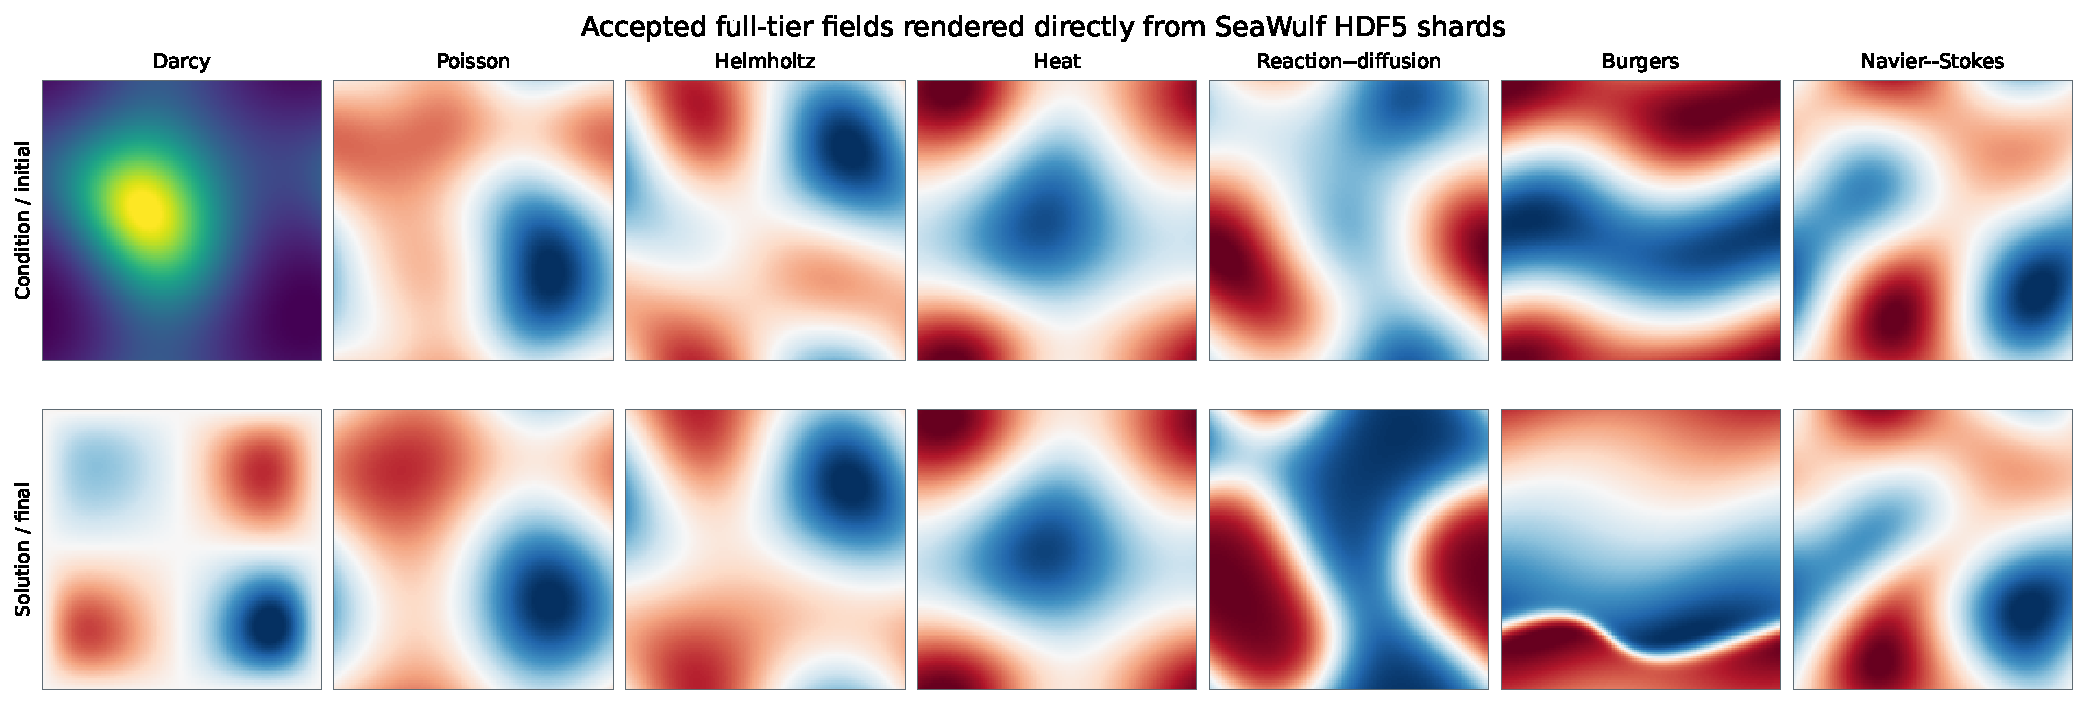
\includegraphics[width=0.96\linewidth]{figures/fig_pde_gallery.pdf}
  \caption{Representative condition/initial and solution/final fields from
  the seven built-in PDE generators.  Every panel is rendered directly from an
  accepted $128\times128$ full-tier HDF5 shard on SeaWulf.  The exact source
  paths and rendering time are recorded in the accompanying machine-readable
  figure snapshot.}
  \label{fig:pde-gallery}
\end{figure}

\subsection{Temporal grids and quality-aware refinement}

The saved trajectory is a view of a denser integration, not the integrator
itself.  In the current full configuration, baseline in-memory grids use 155
frames for heat and 267 for reaction--diffusion and Burgers.  Difficult
Burgers threshold cases use 533.  Navier--Stokes grids vary by topology,
setting, and regime (typically 71--533).  Every count is $1+14q$, so the 15
stored frames are exact solver states selected with a uniform integer stride.

If a sample fails the PDE-loss gate, recovery keeps its factor labels, seed,
physical horizon, and 15 stored times fixed.  Only a documented numerical
route or internal grid may change.  Failed and partial artifacts are moved to a
reversible quarantine; a recovery plan is checked for overlap before
submission.  Repeated time refinement is not assumed to be universally
beneficial: a non-monotone residual indicates that the spatial discretization,
boundary closure, or solver family must be reconsidered instead.

\subsection{Storage, integrity, and reproducibility checklist}

Each accepted shard contains floating-point condition, trajectory, and
geometry arrays in HDF5, plus machine-readable metadata.  Gzip compression and
shuffle are enabled.  The writer flushes to a partial path, computes quality
records, writes sidecars and SHA-256 provenance, and only then publishes the
completed path.  Independent aggregation checks the frozen expected plan,
required PDE coverage, sample rows, completion markers, checksums, failure
logs, and the strict quality ceiling.

For an external reproduction, we recommend reporting:
\begin{enumerate}
  \item repository commit and resolved YAML/JSONL plan;
  \item exact HDF5 and sidecar checksums;
  \item Python/package environment and compute platform;
  \item split, mask, observed count, fit scope, and stochastic seed;
  \item all field, spectral, horizon, physics, and stability metrics required
  by the selected task;
  \item any recovery row and the numerical reason it replaced the original.
\end{enumerate}
These items make the benchmark builder, rather than an informal collection of
files, the auditable source of experimental truth.

\ifdefined\PDEOBSAPPENDIXINPUT
\else
\clearpage
\bibliographystyle{plainnat}
\bibliography{references}

\end{document}
\fi


\end{document}
